%        File: pnas1.tex
%     Created: Wed Apr 30 04:00 pm 2014 E
% Last Change: Wed Apr 30 04:00 pm 2014 E
%
\documentclass[letterpaper]{article} 
\usepackage{aaai} 
\usepackage{times} 
\usepackage{helvet} 
\usepackage{courier} 
\setlength{\pdfpagewidth}{8.5in} 
\setlength{\pdfpageheight}{11in} 
%%%%%%%%%%
% PDFINFO for PDFLATEX
% Uncomment and complete the following for metadata (your paper must compile with PDFLATEX)
\pdfinfo{
	/Title Inter-Task Effects induce Bias in Crowdsourcing
	/Author Edward Newell
	/Keywords priming, framing, micro-task, crowdsourcing
}


\usepackage{scrextend}
\usepackage{graphicx}
\usepackage{amsmath}
\usepackage{amssymb}
\usepackage{mathrsfs}
\usepackage{gensymb}
\usepackage{algorithm2e}
\usepackage{amsthm}

\newtheorem*{mydef}{Definition}

\usepackage{framed, color}
\usepackage{soul}
\usepackage[colorlinks=false, urlcolor=blue]{hyperref}
\usepackage{dcolumn}
\usepackage{multirow}
\usepackage{booktabs}
\newcolumntype{d}{D{.}{.}{4.0}}
\newcolumntype{s}{D{.}{.}{1.4}}

%\setlength{\parindent}{0cm}
%\setlength{\parskip}{4mm plus1mm minus1mm}

%%%%%%%%%%
% Section Numbers
% Uncomment if you want to use section numbers % and change the 0 to a 1 or 2
% \setcounter{secnumdepth}{0} %%%%%%%%%%
\title{Inter-Task Effects induce Bias in Crowdsourcing}
\author{Edward Newell \and Derek Ruths\\
	McGill University, School of Computer Science, Montreal, Canada\\
}
%%%%%%%%%%
% Body of Paper Begins
\begin{document}
\maketitle
\section*{Abstract}
Microtask platforms allow researchers to engage participants quickly and 
inexpensively.
Workers on such platforms probably perform many tasks in succession,
so we investigate interactions between earlier tasks and later ones, which we 
call ``inter-task'' effects.  
Existing research investigates many task design factors, such as 
``framing'', on the quality of responses, but to our knowledge, does not 
address inter-task effects.  
We use a canonical image-labeling task on Amazon Mechanical Turk 
to measure the impact of inter-task and framing effects on the focus and 
specificity of labels that workers provide.
We also introduce an algorithmic definition of priming, which measures the 
worst-case bias introduced into repsonses.
We find that inter-task effects produced a much stronger impact than framing, 
and demonstrate that our novel priming definition yields a generalized 
measure of priming effects when combined with machine learning algorithms.


\section*{Introduction}

Microtask crowdsourcing platforms like Amazon Mechanical Turk (AMT) make it 
possible to submit batches of small tasks to a large pool of human workers, 
who do the tasks for fun, a sense of purpose, and remuneration 
\cite{kazai2013analysis,Antin20122925}.  
Originally used to distribute clerical work, these platforms 
increasingly serve as a fast and cheap means to engage experimental 
participants in a research 
setting \cite{snow2008cheap}.  

The task requester can interact with the platform like a compute server, 
seamlessly 
integrating human and machine computation.  Researchers have put forward the 
term HPU (Human co-Processing Unit), viewing the introduction of 
microtask platforms as a new computing architecture
\cite{5543192}.  

Here, we highlight an important way in which HPUs differ from CPUs, with 
serious implications for the design of tasks.  It is well known that people 
are subject to priming effects 
\cite{BJOP1796,No2007,beller1971priming} and, in particular, task-repetition effects
\cite{Gass1999549,sohn2001task}.  
We investigate the effect that previously completed tasks have on workers'
responses during subsequent ones. We call such effects 
\textit{inter-task priming}.  Inter-task priming would amount to a kind of
\textit{hysteresis}, meaning that HPU output is not only a function of the 
current input, but also of the history of inputs.

There has been considerable investigation into the factors that affect the 
quality and quantity of micro-task completion.  These include the level of 
pay \cite{kazai2013analysis}, training \cite{le2010ensuring}, screening of 
workers \cite{paolacci2010running}, and user-interface design 
\cite{Finnerty2013}.  Research has also investigated \textit{framing}, 
by testing the effects of disclosing the workflow context 
\cite{Kinnaird2012281}, and the purpose of tasks 
\cite{chandler2013breaking}.  To our knowledge, no study has investigated the 
effects of inter-task priming.

To characterize the effects of inter-task priming, we present a novel  
\textit{algorithmic definition of priming}, and a general method 
for measuring priming effects using machine learning algorithms.  
Studies of priming typically focus on the internal psychological 
mechanisms[***], but our definition focuses on the impact that priming has to
the downstream application of human computation.

In the present work, we investigate inter-task priming on the Amazon 
Mechanical Turk platform, using an image-labeling task, one of the most common 
kinds of tasks on that platform [***].  The task requires workers to label ten 
images featuring 
food and culture.  We regard these images as being made up of an 
\textit{initial} and \textit{final set}, but, crucially, there is no
distinction made between these sets, nor any interruption in the flow of tasks 
from the view of the worker.
We vary the initial set of images, while keeping the final set the same to 
analyze the effect that that the initial images have on the labels that 
workers' attribute to the final set.  We measure effects using our novel 
approach, as well as looking for changes in the content of labels and label 
specificity based on an ontology we developed for that purpose.

As a point of comparison, we subject some groups of workers to a kind of
\textit{framing}: we disclose a fictitious, semantically-loaded name for 
the requester funding the tasks.
The names were chosen to suggest the requester's interest in a specific 
aspect of the image content.  We expect this would cause workers 
to provide more labels, and greater specificity, relating to this 
``preferred'' content.

Surprisingly, we find that inter-task effects are much stronger than the 
framing.  Our results show that initial tasks can significantly alter the 
focus of worker's labels.  Interestingly, we find that inter-task
effects can be used to induce greater specificity.  Our results suggest that
workers attribute more specific labels when labeling a series of images that
that are more similar to one another.  This suggests that careful 
consideration should be given to the bundling of tasks when designing a study 
using a microtask platform.

Our analysis also highlights important advantages of our novel definition of 
priming.  Our approach incorporates no prior knowledge about the nature
of the task whatsoever.  In contrast, we also sought to detect priming
based on its direct effects on label content and specificity,
drawing on prior knowledge about the images and label semantics.
Remarkably, while being more general, our definition yields a more sensitive
measure of priming when combined with machine learning algorithms. 
This approach could be applied to detect priming when one does not 
\emph{a priori} know whether any priming has occurred, 
nor what the nature of the effects might be.
\subsection*{An algorithmic definition of priming}
In psychology, the effects of priming are usually measured in terms of a 
change in the  
speed or accuracy of responses in a task, or in the ability to recognize a 
stimulus object (e.g. a spoken word or an image) when the object is noisier, 
fainter, or briefer.  Methods are also employed to measure processes
in the brain of the participant, such as by fMRI.  Our purpose is different: 
we are interested in assessing the ramifications that priming of HPUs could 
have on the applications to which they are employed.
Thus, we choose to define priming effects in terms of the algorithmic 
distinguishability of the content of primed output.

One difficulty in constructing a definition of priming is that there would 
appear to be no defensible notion of a ``neutral'' or ``unprimed state''.  
While arguments could perhaps be made that one treatment or another is 
\textit{more} 
``neutral'', we choose to define priming relatively, and speak of one 
treatment being \textit{differently primed} from another.

From the point of view of applications, the interest of priming is in how it
affects task performance. Thus, we define priming with respect to a task $\mathcal{T}$.  People will always differ in their initial knowledge, specific 
aptitudes, and in many other intrinsic aspects.  Moreover, priming may not be 
``complete'', in the sense that people's experiences before
priming may continue to have residual effects.  Therefore, we define priming 
in relation to populations, which we regard as having stable distributions of
such latent attributes.

To set up the definition, when a population of people $\mathcal{P}$ performs
a task $\mathcal{T}$ thus producing a population of task-outputs $\mathcal{L}$,
we will write $\mathcal{T}(\mathcal{P}) = \mathcal{L}$.

\vspace{2mm}
\begin{mydef}
	\upshape
	Two mutually exclusive populations of people, $\mathcal{P}_0$ and 
	$\mathcal{P}_1$, are uniformly and randomly subsampled from an initial 
	population $\mathcal{P}$, and are exposed to (possibly) different priming 
	treatments. Each population performs a task $\mathcal{T}$, 
	producing task-outputs $\mathcal{T}(\mathcal{P}_0)$ and 
	$\mathcal{T}(\mathcal{P}_1)$.
	These populations are subsampled, producing 
	$P_0 \subset \mathcal{P}_0$ and
	$P_1 \subset \mathcal{P}_1$. A uniform, random bit is chosen, 
	$b\in _R \{0,1\}$, and a single worker $p$ is uniformly and randomly 
	sampled from 
	$\mathcal{P}_b \setminus P_b$.
	We say that $\mathcal{P}_0$ and $\mathcal{P}_1$ 
	\emph{differ in priming by a degree at least $\theta$},
	if there exists a \emph{distinguisher algorithm} $\mathcal{A}$ that takes as input 
	$\langle\mathcal{T}(J)$, $\mathcal{T}(K)$, $\mathcal{T}(\{p\})\rangle$
	and outputs a guess for $b$ with accuracy $\frac{1+\theta}{2}$.  
\end{mydef}

\begin{figure*}
	\centering{
	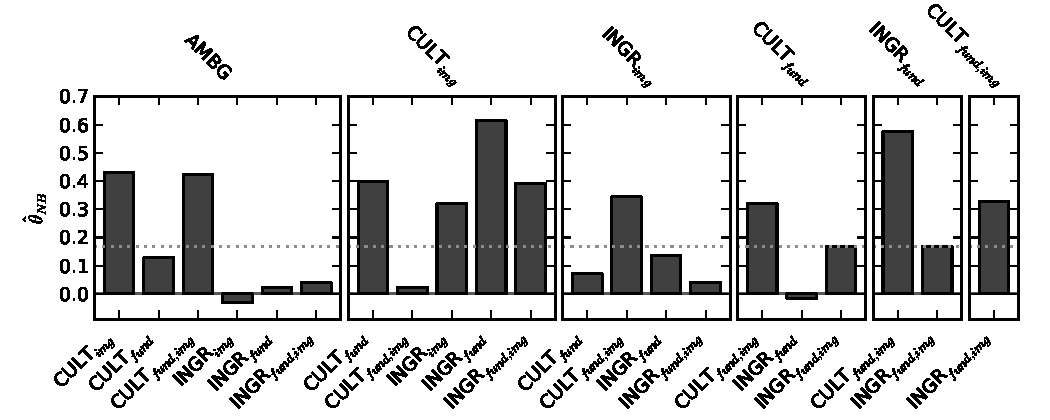
\includegraphics[scale=0.94]{figs/f1-thetas_full_pairwise25_img1.pdf}
	\caption{ \footnotesize{
		Empirical difference in priming, $\hat{\theta}_\text{NB}$, between 
		various treatments.  The difference in priming between each pair of 
		treatments 
		was determined by cross-validation of a Naive Bayes classifier trained
		to classify workers based on the labels they attributed to the first
		image of the final image set. Each panel compares a basis treatment,
		indicated above the panel, to various treatments indicated on the
		abscissa.  We can conclude, with 95\% confidence, that the classifier
		is performing better than chance when $\hat{\theta}_\text{NB}$ 
		exceeds 0.168, indicated by the dotted line.  See \textbf{Methods} for
		the calculation of this confidence threshold.
	}}
}
\end{figure*}

In the language of computer science, $\mathcal{A}$ is a classifier performing
a binary classification.  The measure $\theta$ can range between 0 and 1, and 
indicates how much better the performance of the best possible classifier is 
compared to a random guess. We intentionally leave the details of 
$\mathcal{A}$ unrestricted because the theoretical value of $\theta$ should 
depend on the inherent differences between the populations, rather than on 
the performance of a particular classifier.

In practice, some particular classifier $\mathcal{C}$ is tested (using e.g. 
cross-validation) yielding a statistical estimate of its performance 
$\hat{\theta}_\mathcal{C}$. This
$\hat{\theta}_\mathcal{C}$ acts as a lower bound for the 
theoretical value of $\theta$, because there might 
exist some other classifier $\mathcal{C}'$ with 
$\hat{\theta}_\mathcal{C'}>\hat{\theta}_\mathcal{C}$.
For our experiment, we use a Naive Bayes classifier because it is easy to
implement and performs well across a broad range of classification tasks[***].

To interpret $\hat{\theta}_\mathcal{C}$, imagine that some choice 
$\mathcal{C}$ is to be made between two options on the basis of worker 
outputs (e.g. whether or not to flag an image as inappropriate). Any such 
binary choice has the formal structure of a distinguisher that only considers 
the last of its three inputs. Thus, we can directly compare $\mathcal{C}$ to 
the optimal distinguisher, $\mathcal{A}$.  If, prior to knowing the input to 
$\mathcal{C}$, either of its outcomes is equally likely, then the worst 
possible bias that priming can introduce is bounded above by $\theta$. 
This means that $\hat{\theta}_\mathcal{C}$ estimates a 
lower bound for the worst-case bias introduced in a binary 
decision that provides a full bit of information, made on the basis of worker 
outputs, when one failed to control for the corresponding priming treatments.
\subsection*{Experimental Setup}
\begin{table}[t]
\centering
	\begin{tabular}{ l  l  l }
		\hline                       
		Treatment & Funder & Priming Image Set	\\ 
		\hline                       
		$\textsc{ambg}$ & None & Ambiguous\\
		$\textsc{cult}_{img}$ & None & Cultural\\
		$\textsc{cult}_{fund}$ & Cultural & Cultural\\
		$\textsc{cult}_{fund,img}$ & Cultural & Cultural\\
		$\textsc{ingr}_{img}$ & None & Ingredients\\
		$\textsc{ingr}_{fund}$ & Nutritional & Ingredients\\
		$\textsc{ingr}_{fund, img}$ & Nutritional & Ingredients\\
		\hline  
	\end{tabular}


	\caption{ \footnotesize{ 
		Workers were uniformly randomly assigned to one of the 
		treatments listed above. 
		The full funder names used were 
		``The Global Foundation for Cultural Recognition'' and 
		``The National Foundation for Nutritional Awareness''.  
		The ambiguous, cultural, and ingredients initial image sets are shown 
		in \textbf{Figs. 2}, \textbf{3}, and \textbf{4}.
	}}
	\label{table:1}
\end{table}
We solicited 900 AMT workers to perform an image-labeling task relating to
food and culture.  The workers were randomly assigned to one of seven 
treatments shown in \textbf{Table 1}.  Depending on their treatment, workers were then shown the 
name of a research funder, or this step was skipped.
Next, workers were shown ten images, one at a time and were required to provide
five labels for each.  For the purpose of analysis, we divide the images
into \textit{initial} and \textit{final} sets, comprising respectively the 
first five and last five images.  From the perspective of the worker, there 
was no distinction or interruption between the initial and final sets. 
Depending on the treatment, one of three initial image sets was chosen, but
the final set was always the same.

The final image set, comprised images containing prepared meals and featured a 
prominent, identifiable culture (see \textbf{Fig. 4}).
To identify the initial image sets, we use the names ``ambiguous'', 
``cultural'', and ``ingredients''.  The ambiguous set was chosen to
be similar to the final image set, in the sense that it consisted of
images of prepared meals (see \textbf{Fig. 5}),  but its cultural 
features were less prominent.  The cultural set featured 
iconic cultural scenes, but no food at all (see \textbf{Fig. 6}).  Images from 
the ingredients set depicted separated ingredients, but, 
like the ambiguous set, avoided prominent cultural features (see 
\textbf{Fig. 7}).
\subsection*{Results}
\paragraph{Inter-task priming was strong, while framing was weak.}
We tested for priming effects using our algorithmic definition, implemented 
with a Naive Bayes classifier.  The classifier's accuracy
in cross-validations involving each pair of treatments is shown in 
\textbf{Fig.1}.

With some exceptions, the classifier performed significantly better 
than chance when distinguishing treatments that had different initial tasks.  
This demonstrates that inter-task effects were strong. Of the sixteen 
treatment pairs having different initial tasks, the classifier was unable to
distinguish treatments significantly better than chance in three cases.
Each cases involved distinguishing treatments having the ambiguous and 
ingredients set.  Later we discuss the similarity between image sets, and 
we will argue that this is because the ambiguous and ingredients sets are 
similar.

\begin{figure*}
	\centering{
		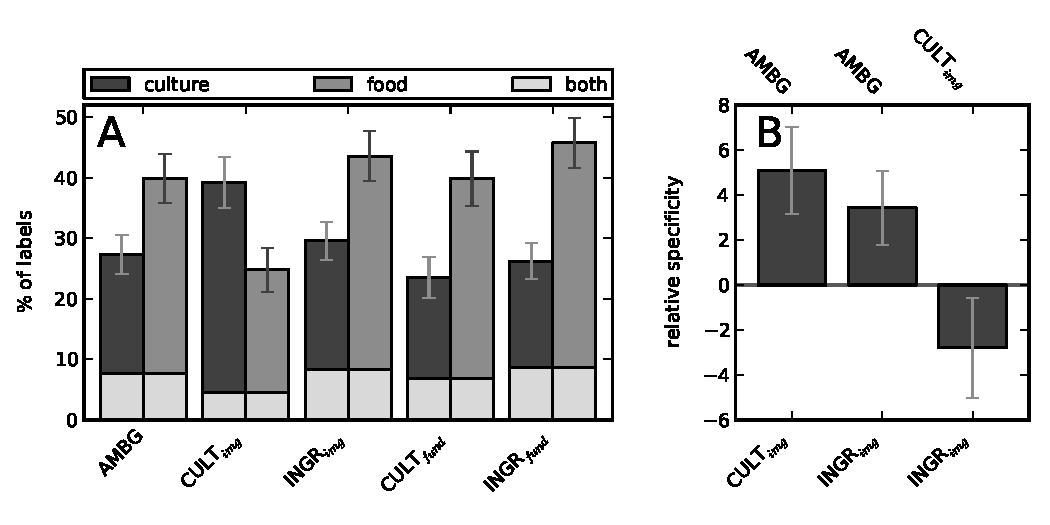
\includegraphics[scale=0.70]{figs/orientation_specificity.pdf}
	\caption{\footnotesize{
		\textbf{A}) Percent label composition (culture- vs food-oriented 
		labels) for 
		various images and treatments.  
		\textbf{B}) Relative specificities of treatments
		indicated along the abscissa compared to those indicated above the 
		plot.  The size of the bar indicates how much more specific
		the labels from one treatment are compared to the other, and points 
		toward in the direction of the more specific treatment.
	}}
}
\end{figure*}
In contrast, the classifier never performed significantly better than chance
when distinguishing treatments that differed only in framing.  Thus, framing 
effects were rather weak.  In fact, framing effects were generally weak in
our results, so we omit treatments involving framing from the remainder of
our presentation to save space.  We encourage the interested reader to look
at the results for these treatments in the supplementary material.
\paragraph{Earlier tasks orient workers' focus during later tasks.} 
Since the initial images were chosen to emphasize either food (ingredients set)
or culture (cultural set), we looked for effects on the number of culture- and 
food-oriented labels that workers attributed to the final image set.

To this end, we constructed an ontology from the labels attributed to the 
test images.  In the ontology, edges point from more general labels to more 
specific ones.  For example, the ontology contains the path \texttt{food} 
$\to$ \texttt{ingredients} $\to$ \texttt{vegetables} $\to$ \texttt{tomato}.
We provide more detail about the construction of the ontology in the 
\textbf{Materials and Methods} section.

Since food is a central feature 
of culture, our ontology contains many labels that have both \texttt{food}
and \texttt{culture} in their ancestry.  Nevertheless, there were many 
food-oriented labels, such as \texttt{bread}, which lacked specific cultural 
connections, as well as non-food, culture-oriented labels, such as 
\texttt{russian dolls}. 

\begin{figure}
	\centering{
	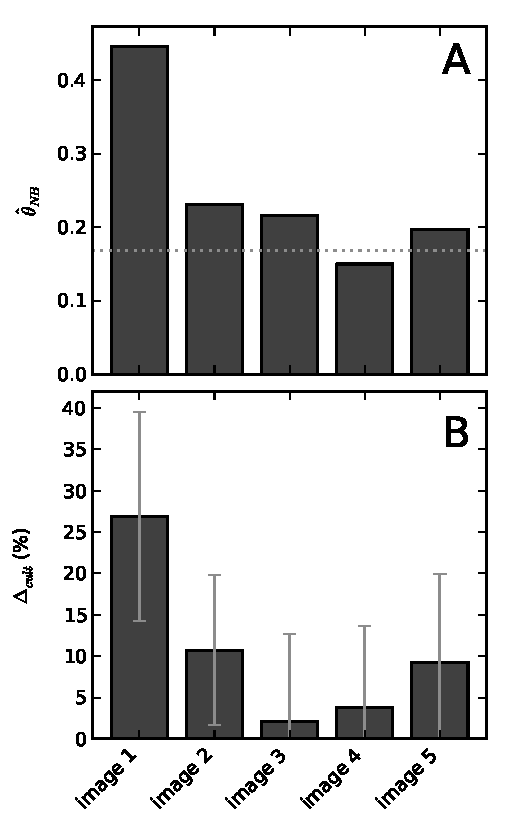
\includegraphics[scale=0.7]{figs/longitudinal_theta_excess-culture.pdf}
	\caption{\footnotesize{
		\textbf{A}) Difference in priming between \textsc{AMBG} and 
		$\textsc{CULT}_{img}$ measured based on the accuracy of a Naive Bayes 
		classifier during cross-validation, when trained on labels from the
		test images indicated along the abscissa.
		\textbf{B}) Excess cultural orientation of labels attributed to
		the test images indicated on the abscissa, by workers from
		$\textsc{CULT}_{img}$ relative to those attributed by workers from
		\textsc{AMBG}, calculated using \textbf{Eq. 3}.
	}}
}
\end{figure}
When we tallied labels attributed to the first image of the final set, 
we found that workers from $\textsc{CULT}_{img}$ produced significantly 
more culture-oriented labels and less food-oriented ones than those from
\textsc{AMBG}
(see \textbf{Fig. 2A}).  The inter-task effect was so strong that the 
proportion of food- and culture-oriented labels in $\textsc{CULT}_{img}$ was
essentially the reverse of that in \textsc{AMBG}.  However, the 
composition of labels attributed by $\textsc{INGR}_{img}$
was not significantly different from those attributed by \textsc{AMBG}.  This 
shows that inter-task effects \textit{can} profoundly alter workers' focus. 
Again, we 
will argue later that the ambiguous and ingredients image sets are, in fact, 
quite similar.
\paragraph{Earlier tasks influenced workers' level of specificity.} 
Using the ontology described in the previous section, we can compare the 
specificity of two labels $\ell_1$ and $\ell_2$. We say that $\ell_2$ is more 
specific than $\ell_1$ if there is a \textit{directed path} from $\ell_1$ to 
$\ell_2$.  If there is no directed path between labels, we say they are  
\textit{non-comparable}.  For example, \texttt{tomato} was more specific than 
\texttt{food}, while \texttt{statue} and \texttt{food} were non-comparable.

We can then define the relative specificity of two workers with respect to 
test-image $i$ as $s_i(u,v)$:

\begin{align}
	s_i(u,v) = \sum_{\ell \in u(i) } \;
	\sum_{m \in v(i)} 
	\left(\mathbf{1}_{[\ell > m]} - \mathbf{1}_{[m>\ell]}\right),
	\label{eq:worker-specificity}
\end{align}
where $u(i)$ denotes the set of labels attributed by worker $u$ to image $i$, 
and $\mathbf{1}_{[\ell > m]}$ evaluates to 1 if $\ell$ is more specific than 
$m$, and 0 otherwise.
We then define the relative specificity of two treatments, $\mathcal{U}$ and 
$\mathcal{V}$, the $i$th image, denoted $S_i(\mathcal{U},\mathcal{V})$, to be 
the mean relative specificity of two uniformly drawn workers:  
\begin{align}
	\hat{S}_i(\mathcal{U},\mathcal{V}) = 
	\frac{1}{|\mathcal{U}| |\mathcal{V}|}
	\sum_{u \in \mathcal{U}} \;
	\sum_{v \in \mathcal{V}} \;
		s_i(u,v).
		\label{eq:specificity}
\end{align}

Looking at labels attributed to the first test image, we found that workers 
from \textsc{AMBG} were more specific than workers from
either $\textsc{CULT}_{img}$ or $\textsc{INGR}_{img}$.  When we compare 
$\textsc{CULT}_{img}$ to $\textsc{INGR}_{img}$, we found that workers from
$\textsc{INGR}_{img}$ were more specific.  This shows that inter-task 
effects do substantially influence the specificity of labels that workers 
provide.  When we discuss image simalarity, below, we will explore a possible
mechanism for this effect.
\paragraph{Inter-task effects ``wash out'' quickly.}  
It would stand to reason that, as workers proceed through the test images, 
priming from the initial images would be ``washed out'', diminishing the 
observed inter-task effects.
Looking at the classifier performance, $\hat{\theta}_\text{NB}$, with respect 
to the treatments \textsc{AMBG} and $\textsc{CULT}_{img}$, we find that 
performance does drop off dramatically after just the first image 
(see \textbf{Fig. 3A}).
This suggests that inter-task effects primarily arise between consecutive 
tasks, but that a residual effect can persist for at least five tasks (we 
note, however that although the classifier performance seemed better than 
chance for the fourth test image, this cannot be asserted with 95\% 
confidence).

Next we observed how inter-task effects on label composition (i.e. food- vs 
culture-orientel labels) evolve as workers proceed through test images.
We define the \textit{excess cultural orientation} as the number of 
culture-oriented labels minus the number of food oriented ones.  To 
meaningfully compare the excess cultural orientation between test images, we 
must, however, account for the fact that some images inherently carry more 
cultural content than others. In keeping with our notion of priming 
\textit{difference}, we calculate the excess cultural content for both 
$\textsc{CULT}_{img}$ and \textsc{AMBG}, and take their difference to be
the \textit{relative} excess cultural content, $\Delta_{cult}$.  Formally,
\begin{align}
	\begin{split}
	\Delta_{cult}(i) = \frac{1}{N}\left[ \sum_{w\in\textsc{cult}_{img}} \left(N_{w,cult}^{(i)} - N_{w,food}^{(i)}\right)\right. \\
\left.	- \sum_{w\in\textsc{ambg}} \left(N_{w,cult}^{(i)} - N_{w,food}^{(i)}\right)\right],
	\end{split}
\end{align}
where $N_{w,cult}^{(i)}$ stands for the number of culture-oriented labels 
attributed by worker $w$ to image $i$, while $N_{w,food}^{(i)}$ similarly 
counts food-oriented labels, and $N$ is the total number of labels in a 
treatment.  

We found $\Delta_{cult}$ was largest for the first test image, but dropped off 
rapidly, remaining positive but not to a statistically significant extent
(see \textbf{Fig. 3B}).  
This is similar to the behavior of $\hat{\theta}_\text{NB}$, however, because
the statistical significance of $\Delta_{cult}$ dropped more quickly, 
$\hat{\theta}_\text{NB}$ appears to be a more sensitive measure of inter-task 
effects.
\paragraph{Inter-task similarity encourages more specific labels.}
To continue with the analysis, we seek a measure of image similarity.  The 
characterization of image content is a deeply complex issue that has been 
approached by many disciplines 
\cite{panofsky1939studies,shatford1986analyzing,Tversky1977327,Jaimes20002}.
\textit{Perceptual similarity} is a particularly recalcitrant concept[***].

However, in the present study, we are more interested how similar two 
sets of images are, \textit{with respect to the labeling task}, which is much
simpler to operationalize than general perceptual similarity.  Here, we 
measure image similarity by looking at the fraction of labels that they share. 
Formally, to measure the similarity between two \textit{sets of images}, $X$ 
and $Y$, we compute the Jacquard index between the sets of labels attributed 
to them:
\begin{align}
	\text{Sim}(X,Y) = \frac{L(X) \cap L(Y)}{L(X) \cup L(Y)},
\end{align}
\begin{table}
\centering
\begin{tabular}{ l  s s s s}

\toprule    
Image set   
& \multicolumn{1}{c}{Ambig.} 
& \multicolumn{1}{c}{Cultural} 
& \multicolumn{1}{c}{Ingr.}
& \multicolumn{1}{c}{Test} \\
  
\midrule

Ambiguous  & 1 & 0.0418 & 0.142 & 0.167 \\

Cultural  & 0.0418  & 1 & 0.0347 & 0.0561 \\

Ingredients  & 0.142  & 0.0347 & 1 & 0.110 \\

Test & 0.167  & 0.0561 & 0.110 & 1
\\
\bottomrule

\end{tabular}
\caption{\footnotesize{
	Number of unique labels attributed to each image set, and their
	similarities based on \textbf{Eq. 4} 
}}
\label{table:2}
\end{table}
where $L(X)$ denotes the set of labels attributed to $X$.

The pairwise similarities of the image sets are presented in \textbf{Table 2}. 
First, observe that the ambiguous and ingredients sets are much more similar 
to each other than either is to the culture set.  Recalling the data presented
in \textbf{Fig. 1}, this helps explain why two treatments could not be 
distinguished on the basis of having differing initial sets corresponding to
ambiguous and cultural.  This also explains why \textsc{ambg} and 
$\textsc{cult}_{img}$ had similar label compositions in \textbf{Fig. 2A}.

Next we draw attention to the similarity between the initial sets and the test 
set.  The ambiguous set is the most similar to the test set, followed by the
ingredients set, with the cultural set being most different.
Observe that these levels of similarity mirror the label specificity for the 
corresponding treatments (c.f. \textbf{Fig. 2B}).  

This suggests that labeling a series of images that are similar to 
one another might encourage workers to use more specific terminology.
Such a phenomenon would be consistent with the psychological mechanism known 
as \textit{negative priming}.  Negative priming occurs when a person becomes 
desensitized to non-salient stimuli to which she is repeatedly 
exposed.  Consider that workers who initially 
labeled the ambiguous image set had already seen five images showing 
prepared meals once they labeled the first test image.  At that point,
a worker might not regard the generic labels \texttt{food} or \texttt{meal} 
to be salient, and opt instead for \texttt{bread}, or \texttt{pasta}.

We are suggesting that, although workers are not instructed to compare
images in any way, prior tasks nevertheless create a frame of reference
relative to which later tasks are judged.  This in turn 
influences the perception of salience. Thus, in a series of subjective 
characterization tasks that have very similar content, workers' focus 
will tend to be directed away from generic, shared attributes, towards those 
attributes that are specific and distinguishing.
\subsection*{Discussion}
\paragraph{Inter-task effects should be considered during task design.}  
Our results show that inter-task effects can have a strong influence on how
workers label images.  In particular, we observed that prior tasks influence
the specificity and content of labels.  Surprisingly, framing a task by 
indicating a semantically-loaded funder had much milder effects on worker 
outputs, generally below the statistical power of our tests.

We therefore caution those designing studies using human computation: even if 
the requester has eliminated surrounding influences to every practical extent, 
\textit{the greatest source of bias might lurk in the tasks themselves}.
Due consideration should be given to how tasks are bundled together.
While our measurements of $\hat{\theta}_\text{NB}$ indicated that inter-task 
effects persisted even to the fifth test image, the most severe effects arise 
between consecutive tasks.
\paragraph{$\theta$ provides a general purpose measure of priming effects.}
When used three approaches to detecting priming effects: 1) using a Naive Bayes
classifier to measure $\hat{\theta}_\text{NB}$, 2) tallying the number of 
culture- and food-oriented labels, and 3) comparing the relative specificity
of labels based on an ontology.  Of the three, measuring $
\hat{\theta}_\text{NB}$ was the most sensitive.  

In one sense, this is not surprising because the Naive 
Bayes classifier takes into account the frequency of occurrence of all labels 
encountered during training.  But it is remarkable that the 
method which incorporates neither prior knowledge about the image contents nor 
label semantics, outperforms those that do.  This is a powerful feature 
because, given the outputs from two sets of workers, one can test whether they 
have been differently primed without knowing how that priming might manifest.

Our algorithmic definition of priming is phrased in terms of worker outputs
rather than psychological phenomena.  This provides a connection between
the priming effects and their potential to impact decisions made on the basis
of worker outputs.  In the case of a binary decision, $\theta$
describes the worst-case bias introduced by failing to control for priming 
effects.
\paragraph{Batching tasks for better HPU performance.}
Our proposed connection between similarity and specificity during 
image-labeling might be used to tune the specificity of labels.  For example,
If one seeks very nuanced labeling, our results suggest that the images 
should first be sorted into batches based on their similarity. This could be 
accomplished by beginning with a first, coarse characterization of unsorted 
images, followed by batching based on the labels obtained. Then, the batches
of similar images could be served for a second round of finer labeling. 
The sorting and re-labeling could then in principle be repeated.

In effect, this creates a hierarchical workflow, where the first, 
coarsely-characterizing HPUs provide a stream of labeled images that is 
split (batched) and fed to other HPUs for finer characterization.  This 
workflow exhibits an interesting difference between HPUs and CPUs.  In general,
whenever an aspect of a problem can be parallelized when employing CPUs, one
gains efficiency.  But here, because of HPU hysteresis, we see an example where
one might sacrifice accuracy through parallelization.
\subsection*{Conclusion}
Inter-task priming can have a strong effect.  
For a canonical image-labeling task, inter-task priming was stronger in its 
effects on the orientation and specificity of labels than was the disclosure of
semantically loaded funder names.  Requesters on microtask platforms should 
take care to avoid introducing biases due to the batching and ordering tasks 
they serve to workers.  At the same time, inter-task priming might be exploited to improve task output, for 
example, to drive more (or less) nuanced responses.

We demonstrated that our algorithmic definition of priming, and its 
implementation using a Naive Bayes classifier, provides a sensitive,
general-purpose method for detecting priming.  Even when the expected effects 
on label orientation and specificity were slight, $\theta_\text{NB}$ 
was significant.  $\theta_\text{NB}$ provides direct statistical evidence that 
populations have been affected by priming, even when the nature of the 
effects are not understood. 
\subsection*{Materials and Methods}
Omitted due to length.  This will be added to supplementary material.
\bibliography{newbib.bib} 
\bibliographystyle{aaai}
\end{document}
\subsection*{Motivation}
I am near the beginning of my PhD studies, and have joined Derek Ruths' lab 
with the expressed purpose of performing human computation research.
My interests lay at the intersection of game theory, psychology, and 
computation.  The overarching goal for my research relates to group 
decisionmaking, and can be phrased in the following way: ``what are the factors
that influence the social efficiency of collective decisionmaking?'' I
view decisionmaking as the central activity of all social organizations, and 
I view this as a computational process.  My reason for 
wanting to attend the PhD Consortium at HCOMP is threefold.  First, I wish to
discuss my ideas with others, get feedback, and learn more about how the 
community frames such questions, to help me as I finalize my PhD proposal 
into concrete research aims.  Second, I hope to make connections to other 
researchers who are interested in similar research questions.  Finally, I wish
to obtain feedback on a crowdsourcing platform that I have implemented (and
hopefully pique other researcher's interest), which I intend to use in my
research.
\end{document}


